
% xetex expected
\documentclass[xetex,professionalfont]{beamer}

% we want math
\usepackage{amsmath}

% fixes and extensions to amsmath
\usepackage{mathtools}

% additional math symbols
\usepackage{amssymb}

% good-looking fractions in text via \sfrac
\usepackage{xfrac}

% fix spaces after custom commands (see below for examples)
\usepackage{xspace}

% minted allows for fancy syntax highlighting (requires python with pygments)
% usage:
%   \begin{minted}{python}
%   codeb
%   \end{minted}
\usepackage{minted}

% better looking tables
% usage:
%   begin with a \toprule, write a single row of column headings,
%   then add \midrule and after the columns of data we finish with \bottomrule
% example:
%   \begin{tabular}{llr} \toprule
%   Animal & Description & Price \midrule
%   cat & foo & 10 \\
%   dog & bar & 20 \\ \bottomrule
%   \end{tabular}
% note that good tables generally neither have vertical rules nor double rules
\usepackage{booktabs}

% system font support (requires xetex or luatex)
\usepackage{fontspec}
\setmonofont[Scale=0.7]{Cousine} % part of ttf-chromeos fonts on Arch

% improve microtypography
\usepackage{microtype}

% multi-language quotes for babel
\usepackage{csquotes}

% easy way to include copyright information
\usepackage{copyrightbox}

% better bibliographies
\usepackage[backend=biber,style=authoryear]{biblatex}

% language support (english,ngerman)
\usepackage[english]{babel}

% -----------------------------------------------------------------------------

% specify PDF metadata
\hypersetup{pdftitle={CVSP VO - IP Recap},pdfsubject={},pdfauthor={Christopher Pramerdorfer}}

% copyright font style
\makeatletter\renewcommand{\CRB@setcopyrightfont}{\tiny\color{lightgray}}

% make emph bold
\DeclareTextFontCommand{\emph}{\bfseries}

% use tuwcvl beamer theme
\usetheme{tuwcvl}

% add bib file
\addbibresource{literature.bib}

% -----------------------------------------------------------------------------

% common english abbreviations
\newcommand{\ie}{\mbox{i.e.}\xspace} % i.e.
\newcommand{\eg}{\mbox{e.g.}\xspace} % e.g.

% math - argmin and argmax
\DeclareMathOperator*{\argmin}{arg\,min}
\DeclareMathOperator*{\argmax}{arg\,max}

% shortcuts for number ranges
\newcommand{\NN}{\mathbb{N}}
\newcommand{\ZZ}{\mathbb{Z}}
\newcommand{\QQ}{\mathbb{Q}}
\newcommand{\RR}{\mathbb{R}}

% bold vectors
\renewcommand{\vec}[1]{\ensuremath{\mathbf{#1}}}

% vector shortcuts
\newcommand{\va}{\vec{a}}
\newcommand{\vb}{\vec{b}}
\newcommand{\vc}{\vec{c}}
\newcommand{\ve}{\vec{e}}
\newcommand{\vr}{\vec{r}}
\newcommand{\vs}{\vec{s}}
\newcommand{\vt}{\vec{t}}
\newcommand{\vu}{\vec{u}}
\newcommand{\vv}{\vec{v}}
\newcommand{\vw}{\vec{w}}
\newcommand{\vx}{\vec{x}}
\newcommand{\vy}{\vec{y}}
\newcommand{\vz}{\vec{z}}

\newcommand{\vX}{\vec{X}}

% -----------------------------------------------------------------------------

\title{Computer Vision Systems Programming VO}
\subtitle{A Recap of Image Processing}
\author{Christopher Pramerdorfer}
\institute{Computer Vision Lab, Vienna University of Technology}

\begin{document}

% -----------------------------------------------------------------------------

\begin{frame}
\maketitle
\end{frame}

% -----------------------------------------------------------------------------

\begin{frame}
\frametitle{Topics}

A brief recap of Image Processing (IP)
\begin{itemize}
	\item Assuming you are already familiar with IP
	\item Focus on methods that are widely used in practice
\end{itemize}

\medskip
\begin{center}
	\copyrightbox[b]
	{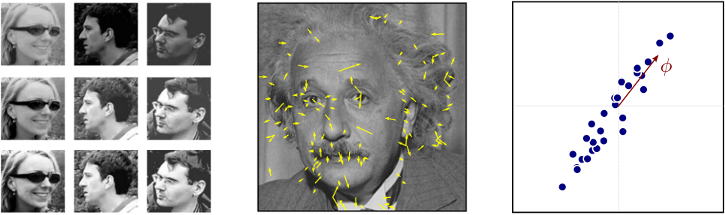
\includegraphics[width=8cm]{figures/intro-collage.png}}
	{\centering Images from \cite{prince12}}
\end{center}

\end{frame}

% -----------------------------------------------------------------------------

\begin{frame}
\frametitle{Relation of IP and CV}

IP encompasses operations that
\begin{itemize}
	\item Take images as input
	\item Produce images or representations (\eg descriptors)
\end{itemize}

\medskip
We regard IP as preprocessing for CV
\begin{itemize}
	\item IP has great influence on CV performance
\end{itemize}

\end{frame}

% -----------------------------------------------------------------------------

\begin{frame}
\frametitle{Relation of IP and CV}

CV is all about
\begin{itemize}
	\item Infering some world state $\vw$
	\item From measurements $\vx$
\end{itemize}

\bigskip
We use IP to obtain a suitable $\vx$ from images % in some tasks x are actual images

\bigskip
Suitable often means
\begin{itemize}
	\item Distinctive features % e.g. descriptors
	\item That are robust and covariant % see Tuytelaars08 for covariance vs invariance
\end{itemize}

\end{frame}

% -----------------------------------------------------------------------------

\begin{frame}
\frametitle{Contrast Normalization}

Reduce variation due to contrast and intensity changes

\bigskip
We cover two techniques
\begin{itemize}
	\item Whitening
	\item Histogram equalization
\end{itemize}

\medskip
\begin{center}
	\copyrightbox[b]
	{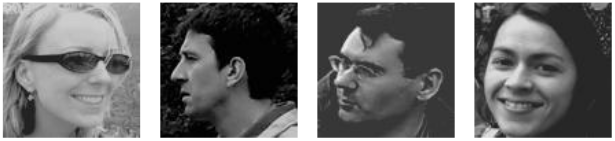
\includegraphics[width=8cm]{figures/contrast-original.png}}
	{\centering Images from \cite{prince12}}
\end{center}

\end{frame}

% -----------------------------------------------------------------------------

\begin{frame}
\frametitle{Contrast Normalization}
\framesubtitle{Whitening}

Transform pixel values so that
\begin{itemize}
	\item Their mean is zero
	\item Their variance is one % i.e. the resulting values are floats. if required, the result can be mapped to [0, 255] again by mapping -1 to 0 and 1 to 255, for example
\end{itemize}

\medskip
\begin{center}
	\copyrightbox[b]
	{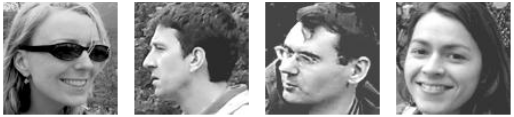
\includegraphics[width=8cm]{figures/contrast-whitening.png}}
	{\centering Images from \cite{prince12}}
\end{center}

\end{frame}

% -----------------------------------------------------------------------------

\begin{frame}[fragile]
\frametitle{Contrast Normalization}
\framesubtitle{Whitening -- Matlab Implementation}

\begin{minted}{matlab}
img = single(rgb2gray(imread('image.png'))); % load
m = mean(img(:)); % compute mean
s = std(img(:)); % compute standard deviation
whitened = (img - m) / s; % normalize
\end{minted}

\end{frame}

% -----------------------------------------------------------------------------

\begin{frame}
\frametitle{Contrast Normalization}
\framesubtitle{Histogram equalization}

Transform pixel values so that distribution is \enquote{flat} % not exactly flat because input is descrete (see example images on Wikipedia)
\begin{itemize}
	\item Cumulative histogram linear over value range % like 0 ... 255 in 8-bit case
\end{itemize}

\medskip
\begin{center}
	\copyrightbox[b]
	{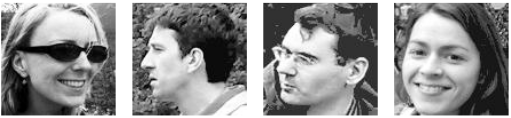
\includegraphics[width=8cm]{figures/contrast-histeq.png}}
	{\centering Images from \cite{prince12}}
\end{center}

\end{frame}

% -----------------------------------------------------------------------------

\begin{frame}[fragile]
\frametitle{Contrast Normalization}
\framesubtitle{Histogram Equalization -- C++ Implementation}

\begin{minted}{cpp}
// cv = OpenCV namespace
cv::Mat img, equalized; // storage
img = cv::imread("image.png", cv::IMREAD_GRAYSCALE); // load
cv::equalizeHist(img, equalized); // normalize
\end{minted}

\end{frame}

% -----------------------------------------------------------------------------

\begin{frame}
\frametitle{Noise Reduction and Change Detection}

Reduce image noise\\\medskip
Locate intensity changes

\bigskip
Often accomplished via \emph{linear filtering}
\begin{itemize}
	\item Pixel values linear combination of neighbor values
	\item Computed via convolution (or correlation)
\end{itemize}

\[
f'(x,y) = \sum_{i,j}f(x-i,y-j)h(i,j) % with convolution the kernel is flipped (x-i,y-j), with correlation this is not the case (x+i,y+j) ... most IP kernels are symmetric so the result is the same
\]

\end{frame}

% -----------------------------------------------------------------------------

\begin{frame}
\frametitle{Noise Reduction and Change Detection}
\framesubtitle{Noise Reduction via Blurring}

Use a 2D Gaussian as kernel $h$:
\[
h(i,j)=\frac{1}{2\pi\sigma^2}\exp\left(-\frac{i^2+j^2}{2\sigma^2}\right)
\]

\begin{center}
	\copyrightbox[b]
	{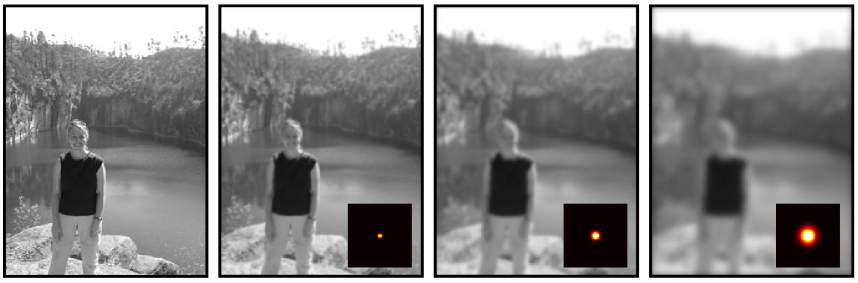
\includegraphics[width=8cm]{figures/linear-blur.png}}
	{\centering Images from \cite{prince12}}
\end{center}

\end{frame}

% -----------------------------------------------------------------------------

\begin{frame}[fragile]
\frametitle{Noise Reduction and Change Detection}
\framesubtitle{Noise Reduction via Blurring -- Matlab Implementation}

\begin{minted}{matlab}
img = rgb2gray(imread('image.png')); % load
h = fspecial('gaussian', [3 3], 0.5); % create Gaussian kernel
filtered = imfilter(img, h); % filter
\end{minted}

\end{frame}

% -----------------------------------------------------------------------------

\begin{frame}
\frametitle{Noise Reduction and Change Detection}
\framesubtitle{Change Detection via LoG Filtering}

Use a Laplacian of Gaussian (LoG) filter as kernel $h$ % for 3x3 this is just [0 -1 0 ; -1 4 -1 ; 0 -1 0]
\begin{itemize}
	\item Gaussian for noise reduction
	\item Laplacian approximates $\nabla^2=f_{xx}+f_{yy}$ % sum of second unmixed derivatives of image
\end{itemize}

\bigskip
LoG filters respond to intensity changes % strong response near corners, zero crossing on corners
\begin{itemize}
	\item Regardless of direction
	\item At a frequency defined by $\sigma$ of Gaussian
\end{itemize}

\bigskip
Substrate for SIFT interest points % SIFT actually used differences of Gaussians to approximate LoG, which is faster

\end{frame}

% -----------------------------------------------------------------------------

\begin{frame}
\frametitle{Noise Reduction and Change Detection}
\framesubtitle{Change Detection via LoG Filtering}

\begin{center}
	\copyrightbox[b]
	{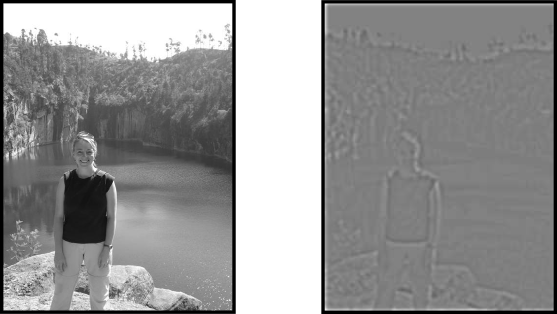
\includegraphics[width=7cm]{figures/linear-log.png}}
	{\centering Images from \cite{prince12}}
\end{center}

\end{frame}

% -----------------------------------------------------------------------------

\begin{frame}[fragile]
\frametitle{Noise Reduction and Change Detection}
\framesubtitle{Change Detection via LoG Filtering -- Matlab Implementation}

\begin{minted}{matlab}
img = rgb2gray(imread('image.png')); % load
h = fspecial('log', [3 3], 0.5); % create LoG kernel
filtered = imfilter(img, h); % filter
\end{minted}

\end{frame}

% -----------------------------------------------------------------------------

\begin{frame}
\frametitle{Noise Reduction and Change Detection}
\framesubtitle{Change Detection via Gabor Filtering}

Use a Gabor filter as kernel $h$, which consists of
\begin{itemize}
	\item A Gaussian for noise reduction
	\item A Sinusoid for change detection 
\end{itemize}

\bigskip
Gabor filters respond to intensity changes at a
\begin{itemize}
	\item Phase and orientation defined by the Sinusoid % phase, orientation, wavelength, but can be made independent of phase by summing squared responses of two filters with pi/2 phase shift
	\item Frequency defined by the Gaussian and Sinusoid
\end{itemize}

\bigskip
Substrate for object recognition and scene understanding

\end{frame}

% -----------------------------------------------------------------------------

\begin{frame}
\frametitle{Noise Reduction and Change Detection}
\framesubtitle{Change Detection via Gabor Filtering}

\begin{center}
	\copyrightbox[b]
	{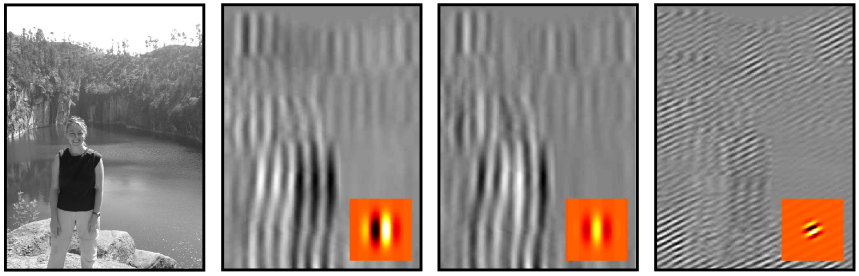
\includegraphics[width=10cm]{figures/linear-gabor.png}}
	{\centering Images from \cite{prince12}}
\end{center}

\end{frame}

% -----------------------------------------------------------------------------

\begin{frame}[fragile]
\frametitle{Noise Reduction and Change Detection}
\framesubtitle{Change Detection via Gabor Filtering -- C++ Implementation}

% OpenCV does not provide LoG filters, so we can either create them by
% convolving a Gaussian and a Laplacian or we can apply both filters consecutively
% this is possible because convolution is associative

\begin{minted}{cpp}
cv::Mat img, gabor; // storage
img = cv::imread("image.png", cv::IMREAD_GRAYSCALE); // load
h = cv::getGaborKernel(...); // create Gabor kernel
cv::filter2D(img, gabor, CV_32F, h); // filter

\end{minted}

\end{frame}

% -----------------------------------------------------------------------------

\begin{frame}
\frametitle{Interest Point Detection}

Interest points are image features that
\begin{itemize}
	\item Are local (precise location, little spatial extent) % at the end they are just points (precise location (up to subpixel) and no extent), but since they are computed from a local neighborhood, they have an implicit spatial extent (see Tuytelaars08)
	\item Can be detected reliably in multiple images of same object % i.e. high repeatability
\end{itemize} % this is not a complete definition, see Tuytelaars08 for more information

\bigskip
Which implies that they are
\begin{itemize}
	\item Invariant to image transformations
	\item Robust with respect to noise
\end{itemize}

\end{frame}

% -----------------------------------------------------------------------------

\begin{frame}
\frametitle{Interest Point Detection}
\framesubtitle{Harris Corner Detector}

Corners characterized by intensity change in multiple directions

\bigskip
Harris corner detector exploits this by
\begin{itemize}
	\item Checking gradient distribution in local neighborhood
	\item Corner: gradient distribution has two large eigenvalues
\end{itemize}

\begin{center}
	\copyrightbox[b]
	{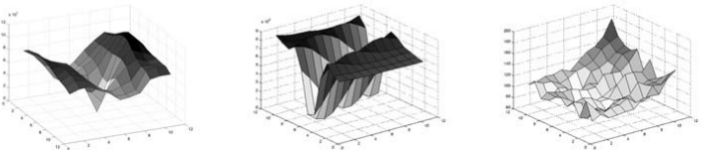
\includegraphics[width=10cm]{figures/cornerness.png}}
	{\centering Images from \cite{szeliski2010}}
\end{center}

\end{frame}

% -----------------------------------------------------------------------------

\begin{frame}
\frametitle{Interest Point Detection}
\framesubtitle{Harris Corner Detector}

Harris interest points
\begin{itemize}
	\item Are invariant to translation and rotation
	\item Stable under varying lighting conditions % because they are based on derivatives
\end{itemize} % they are also among the most repeatable and most informative, see Tuytelaars08

\medskip
\begin{center}
	\copyrightbox[b]
	{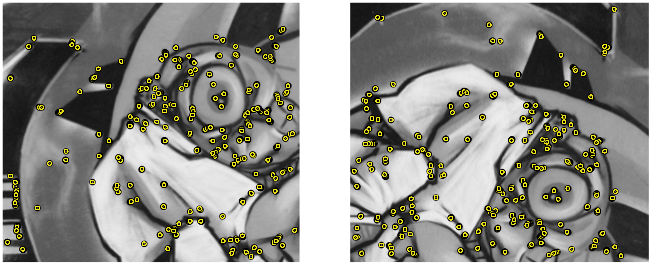
\includegraphics[width=8cm]{figures/ip-harris.png}}
	{\centering Images from \cite{tuytelaars2008}}
\end{center}

\end{frame}

% -----------------------------------------------------------------------------

\begin{frame}[fragile]
\frametitle{Interest Point Detection}
\framesubtitle{Harris Corner Detector -- Matlab Implementation}

\begin{minted}{matlab}
img = rgb2gray(imread('image.png')); % load
corners = corner(img, 'Harris', maxNum); % detect corners
\end{minted}

\end{frame}

% -----------------------------------------------------------------------------

\begin{frame}
\frametitle{Interest Point Detection}
\framesubtitle{SIFT Detector}

Scale invariant blob detector
\begin{itemize}
	\item A blob is an image region with similar intensity % surrounded by regions with different intensity, again see Tuytelaars08 for more information
\end{itemize}

\bigskip
Blob detection accomplished via LoG filtering
\begin{itemize}
	\item LoG filter responds to blobs of size that depends on $\sigma$
\end{itemize}

\bigskip
Scale invariance is achieved by
\begin{itemize}
	\item Applying LoG filter with multiple $\sigma$
	\item Finding local maxima in resulting scale-space
\end{itemize}

\bigskip
Repeated LoG approximated by Differences of Gaussians (DoGs)

\end{frame}

% -----------------------------------------------------------------------------

\begin{frame}
\frametitle{Interest Point Detection}
\framesubtitle{SIFT Detector -- Scale Space}

\begin{center}
	\copyrightbox[b]
	{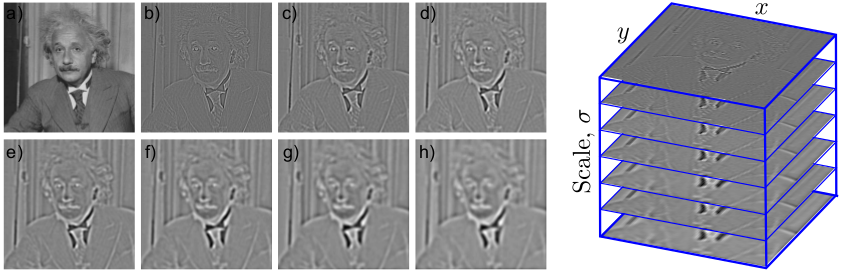
\includegraphics[width=10cm]{figures/sift-scale-space.png}}
	{\centering Images from \cite{prince12}}
\end{center}

\end{frame}

% -----------------------------------------------------------------------------

\begin{frame}
\frametitle{Interest Point Detection}
\framesubtitle{SIFT Detector}

Local maxima are
\begin{itemize}
	\item Localized to sub-voxel accuracy % via Taylor expansion, which leads to a more accurate position and scale estimation, see Prince's book
	\item Discarded unless on corners % corners in the above sense, not necessarily actual corners
	\item Assigned an orientation via gradient histograms % multiple keypoints are generated if there are more several dominant orientations
\end{itemize}

\begin{center}
	\copyrightbox[b]
	{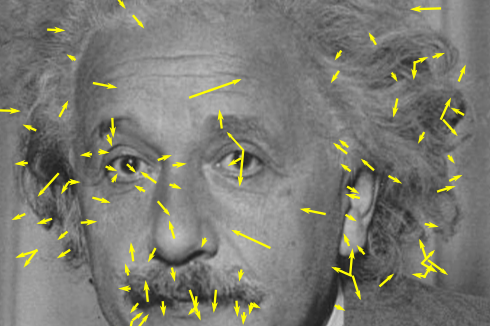
\includegraphics[width=4cm]{figures/ip-sift.png}}
	{\centering Image from \cite{prince12}}
\end{center}

\end{frame}

% -----------------------------------------------------------------------------

\begin{frame}[fragile]
\frametitle{Interest Point Detection}
\framesubtitle{SIFT Detector -- C++ Implementation}

% first argument to sift detector is minimum magnitude of scale-space maxima.
% second argument to sift detector is the minimum determinant of the Hessian,
% which is used to discard non-corner keypoints.

\begin{minted}{cpp}
cv::Mat img = cv::imread("image.png", cv::IMREAD_GRAYSCALE);
cv::SiftFeatureDetector det(20, 10); // create detector
std::vector<cv::KeyPoint> kps; // keypoint storage
det.detect(img, kps); // detect keypoints
\end{minted}

\end{frame}

% -----------------------------------------------------------------------------

\begin{frame}
\frametitle{Local Descriptors}

Compact representations of contents of an image region\\\medskip
Usually computed at interest point locations\\\medskip % but dense representations have uses as well
Invariant in conjunction with suitable interest points\\\medskip % see next slide
Pool information locally to achieve robustness % wrt. small spatial transformations / tradeoff between preserving spatial information and robustness
\begin{itemize}
	\item Often accomplished via histograms
\end{itemize}

\end{frame}

% -----------------------------------------------------------------------------

\begin{frame}
\frametitle{Local Descriptors}
\framesubtitle{SIFT Descriptor}

Computed from gradient histograms\\\medskip
Usually used together with SIFT interest points
\begin{itemize}
	\item Compensate for scale, rotation % by transforming image patch by interest point properties before computing descriptors
\end{itemize}

\begin{center}
	\copyrightbox[b]
	{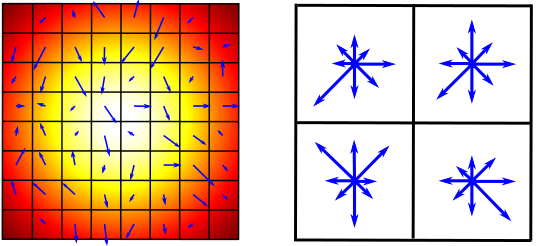
\includegraphics[width=6cm]{figures/sift-descriptor.png}} % divide 8x8 pixel grid into 2x2 cells, pool directions in each cell using a histogram with 8 bins (sift uses 16x16 patches and 4x4 cells, so we have 4x4x8=128 values per descriptor, which is then normalized)
	{\centering Images from \cite{prince12}}
\end{center}

\end{frame}

% -----------------------------------------------------------------------------

\begin{frame}
\frametitle{Local Descriptors}
\framesubtitle{SIFT Descriptor}

SIFT descriptors are
\begin{itemize}
	\item Invariant to scale and rotation (interest points)
	\item Invariant to global intensity changes (gradients)
	\item Robust to small affine transformations (pooling)
\end{itemize}

\end{frame}

% -----------------------------------------------------------------------------

\begin{frame}[fragile]
\frametitle{Local Descriptors}
\framesubtitle{SIFT Descriptor -- C++ Implementation}

\begin{minted}{cpp}
// img and kps from previous example
cv::Mat descriptors; // storage (n by 128)
cv::SiftDescriptorExtractor ex; // create extractor
ex.compute(img, kps, descriptors); // compute descriptors
\end{minted}

\end{frame}

% -----------------------------------------------------------------------------

\begin{frame}
\frametitle{Dimensionality Reduction}

Sometimes desirable to reduce the dimensionality of $\vx$
\begin{itemize}
	\item Makes learning and inference more efficient
	\item Can improve generalization performance % same number of measurements, smaller feature dimensionality can improve generalization performance in absence of regularization
	\item Facilitates data visualization
\end{itemize} % see Webb11 for more information

\bigskip
Goal is to find transformation from $\vx$ to $\vv$
\begin{itemize}
	\item With $v=\dim(\vv)<x=\dim(\vx)$
	\item That minimizes the information loss
\end{itemize}

\end{frame}

% -----------------------------------------------------------------------------

\begin{frame}
\frametitle{Dimensionality Reduction}
\framesubtitle{Principal Component Analysis}

Principal Component Analysis (PCA) yields
\begin{itemize}
	\item The orthogonal transformation $\phi$ to a $v$-dimensional subspace
	\item That minimizes $\sum_i\lVert\vx_i-\phi^{-1}\vv_i\rVert_2$ (assuming zero mean) % the squared reconstruction error / transformation is orthogonal so phi is a matrix and phi^-1 = phi^T / note that the notation is the other way around in Prince's book / in practice, zero mean is enforced by subtracting the empirical mean from all x
\end{itemize}

\bigskip
Accomplished if $\phi=[\phi_1,\dots,\phi_v]^T_{v\times x}$ % again, assuming zero mean
\begin{itemize}
	\item With $\phi_k$ being the $k$th largest eigenvectors of $\vX\vX^T$
	\item Where $\vX=[\vx_1,\dots,\vx_I]$
\end{itemize}

\bigskip
Projects $\vx_i$ onto hyperplane
\begin{itemize}
	\item Spanned by $v$ largest axes of covariance ellipsoid
\end{itemize}

\end{frame}

% -----------------------------------------------------------------------------

\begin{frame}
\frametitle{Dimensionality Reduction}
\framesubtitle{Principal Component Analysis -- Example}

In this case $h=v$ and $\phi=\phi^{-1}=\phi^T$

\begin{center}
	\copyrightbox[b]
	{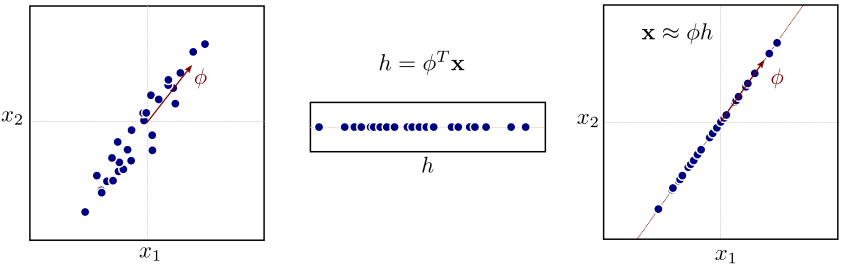
\includegraphics[width=10cm]{figures/pca.png}} % TODO adapt to text notation
	{\centering Images from \cite{prince12}}
\end{center}

\end{frame}

% -----------------------------------------------------------------------------

\begin{frame}
\frametitle{Dimensionality Reduction}
\framesubtitle{Principal Component Analysis -- Remarks}

PCA is dependent on the units of $x_i$
\begin{itemize}
	\item So standardize (whiten) your data % see beginning of slides
\end{itemize}

\bigskip
PCA is unsupervised and linear
\begin{itemize}
	\item Better methods for supervised case (\eg LDA) % check the fisherfaces paper, which illustrates this well
	\item More powerful non-linear methods (\eg autoencoders)
	\item But generally superfluous with modern learning methods % SVMs, random forests etc. include means for regularization and feature selection and are thus robust wrt. feature dimension and redundancy
\end{itemize}

\end{frame}

% -----------------------------------------------------------------------------

\begin{frame}[fragile]
\frametitle{Dimensionality Reduction}
\framesubtitle{Principal Component Analysis -- Matlab Implementation}

% Matlab assumes that each row is a measurement, we assume each column is one

\begin{minted}{matlab}
pc = princomp(X'); % compute all principal components (sorted)
phi = c(:,1:v)'; % keep only v "largest" ones and transpose
V = phi * X; % project to lower dimension
Xe = phi' * V % reconstruct X
\end{minted}

\end{frame}

% -----------------------------------------------------------------------------

\begin{frame}
\frametitle{Summary}

We utilize IP to obtain $\vx$ from an image
\begin{itemize}
	\item That is for feature extraction
\end{itemize}

\bigskip
We want $\vx$ to be distinctive, invariant, robust, concise
\begin{itemize}
	\item And we have seen methods to achieve this
\end{itemize}

\bigskip
We have only scratched the surface of IP
\begin{itemize}
	\item See literature
\end{itemize}

\end{frame}

% -----------------------------------------------------------------------------

\begin{frame}
\frametitle{Bibliography}

\printbibliography

\end{frame}

\end{document}